%Template by Mark Jervelund - 2015 - mjerv15@student.sdu.dk

\documentclass[a4paper,10pt,titlepage]{report}

\usepackage[utf8]{inputenc}
\usepackage[T1]{fontenc}
\usepackage[english]{babel}
\usepackage{amssymb}
\usepackage{amsmath}
\usepackage{amsthm}
\usepackage{graphicx}
\usepackage{fancyhdr}
\usepackage{lastpage}
\usepackage{pgfplots}
\usepackage{listings}
\usepackage{algorithm}
\usepackage{algpseudocode}
\usepackage{wrapfig}
\usepackage[document]{ragged2e}
\usepackage[margin=1in]{geometry}
\usepackage{enumitem}
\usepackage{color}
\usepackage{datenumber}
\usepackage{venndiagram}
\usepackage{chngcntr}
\setdatetoday
\addtocounter{datenumber}{0} %date for dilierry standard is today
\setdatebynumber{\thedatenumber}
\date{}
\setcounter{secnumdepth}{0}
\pagestyle{fancy}
\fancyhf{}


%lstlisting ting:
\definecolor{dkgreen}{rgb}{0,0.45,0}
\definecolor{gray}{rgb}{0.5,0.5,0.5}
\definecolor{mauve}{rgb}{0.30,0,0.30}
\lstset{frame=tb,
  language=C++,
  aboveskip=3mm,
  belowskip=3mm,
  showstringspaces=false,
  columns=flexible,
  basicstyle={\small\ttfamily},
  numbers=left,
  numberstyle=\footnotesize,
  keywordstyle=\color{dkgreen}\bfseries,
  commentstyle=\color{dkgreen},
  stringstyle=\color{mauve},
  frame=single,
  breaklines=true,
  breakatwhitespace=false
  tabsize=1
}
\renewcommand{\lstlistingname}{Code}

\newcommand{\Z}{\mathbb{Z}}
\lhead{Parallel Computinge (DM818))}
\rhead{Mark Jervelund (Mjerv15)}
\rfoot{Page  \thepage \, of \pageref{LastPage}}
\counterwithin*{equation}{section}

\begin{document}
\begin{titlepage}
\centering
    \vspace*{9\baselineskip}
    \huge
    \bfseries
    1. Mandatory Assignment \\
    \normalfont
    Mark Jervelund  \\
    (Mjerv15) \\
	\huge
    Parallel Computing (DM818)  \\[4\baselineskip]
    \normalfont
	
\includegraphics[scale=1]{SDU_logo}
    \vfill\
    \vspace{5mm}
    IMADA \\

    \textbf{\datedate}  \bf{at 10} \\[2\baselineskip]
\end{titlepage}

\renewcommand{\thepage}{\roman{page}}% Roman numerals for page counter
\tableofcontents
\newpage
\setcounter{page}{1}
\renewcommand{\thepage}{\arabic{page}}


\section{Introduction}

for the 2nd project in DM818 the task is to optimize and then parallelize a particle simulator.\\ For starting out we were given codes for a basic


\subsection{Work load}


\subsection{Issues}


\section{Design}

\subsection{Binning}
\begin{wrapfigure}{r}{0.25\textwidth} %this figure will be at the right
    \centering
    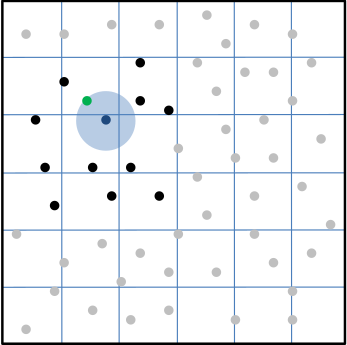
\includegraphics[width=0.25\textwidth]{grid.png}
\end{wrapfigure}
The binning algorithm was designed to make use of a grid, so it could work the same way af the matric matrix blocking where it would interact with index +(-1,-1), to (1,1). \\

With a design like this elements can be dynamiclly removed and added which should remove the computational waste of clearing the grid and reinitinaling it. it also allows the grid to be cleared on every cycle if it is needed. \\

\subsection{Serial with grid}
The serial grided implmentation is designed so it will only need itself and the 8 grids surounding it to calculate the forces needed to move the particle.

\subsection{OPENMP with grid}
For designing the openmp implementaiton the gridded implementation was used as a starting point and the loops with applyforce and move should be made parallel. the grid\_clear will have to have a barrier so threads won't start adding elements to the old grid that will be cleared by the main process. this will most likely cause some overhead.

\subsection{MPI with grid}

The reasosning behind a mpi implmentation is to split the grid into smaller chunks, this can be done in a few different ways, the most aparent is splitting the chucks into smaller squres, but this requires the larger grid to be divisable by p, a different aproch is to split the grid into rows. \\
For the sub cubed inplementation we'll have to talk to the 8 surounding threads which could induce a huge commnunication overhead, while the row wise implementaiton only required the threads to talk to 2 threads, and 1 for the top and lowest thread. \\

The commnucation per step would for each process be 2 x gridwidth x size of particle\_t. this is reasonable but at everystep we'd need to sync so all threads have the required data. \\

\newpage

\section{Implementation}
\subsection{grid}
The implemenation of grid.cpp has a few small functions. the most important one being the get Neighbors functions. This returns the surounding cells to the particle we wish to calculate the forces for. to The grid is stored as an array so to return the currect cell we use the same calculation as we need with the blocked matrix matrix program
\begin{equation}
index = currect location + row + column * rowlengt
\end{equation}
The other functions of the grid that are of some important is the clear and add function. i also implemented a remove element since it was mentionionged the other implementaion could slow execution down, but as i was unble to get it to work i used the clear function.

\subsection{Serial grid}

The optimized serial implementation was modified by modifying the compute forces loops to work in a blocked manner. this was simply done by adding 2 for loops that go from index x-1 y-1 to x+1 y+1 and a inner loop the loops over all particles in those grids.\\
The move part of the code was modified by first clearing the grid as i was unable to get the computation to work currectly when just removing the element. and then calling the move function from common and adding the particle with its new values to the grid. 

\subsection{OPENMP grid}
The paraliesable area in the openmp implementation is all the code surounding the main step for loop. Whats made paralelle here is the apply force loop. this is done using \#pragma omp for, futhermore a \#pragma omp barrier is put in front of this here to make sure the master thread is done saving the data before other threads start using it. \\

The move loop is is made so only a single thread is doing this. when it was using multiple threads there was some issues with segmentation faults and unstability. \\

\subsection{mpi grid}
The mpi im


\section{Testing \& issues}

\subsection{Serial with grid}
The implemented gridded version seems to run within the constriains of the included correction code.

\subsection{openmp with grid}
The openmp verstion was working the other day, i changed something and now it's broken


\section{Comparison}

\subsection{Serial}
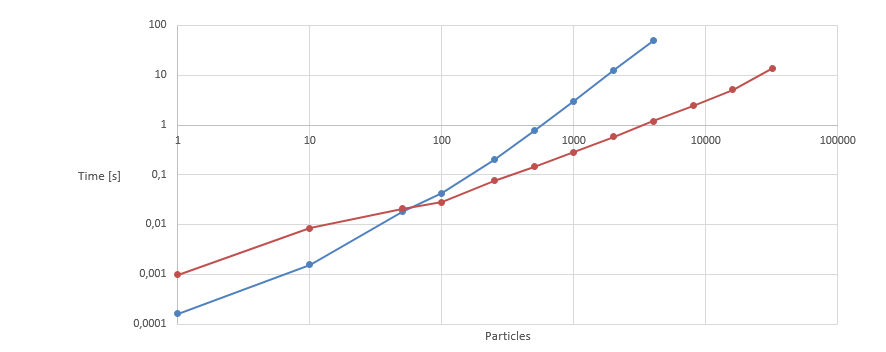
\includegraphics[scale=0.3]{oldvsnew}

\subsection{Openmp}

\subsection{MPI}

\section{Conclusion}
\newpage
\section{appendix}
\subsection{data}
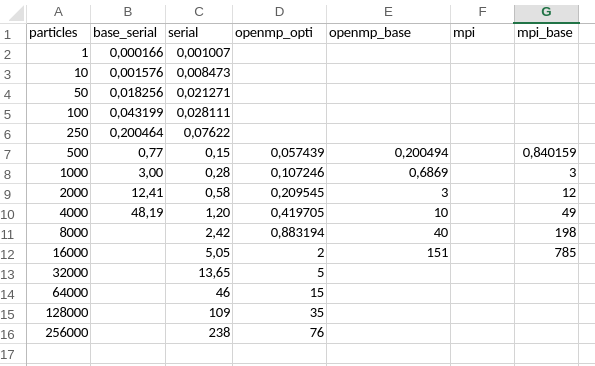
\includegraphics[scale=0.7]{alldata}

\section{Code}

%\lstinputlisting{../src/dgemm.cpp}

%\lstinputlisting{../src/test.cpp}

\end{document}

